\chapter{函数的极限}
\label{chap:function-limits}
\label{chap:mathematical-analysis}

第~\ref{chap:sets-functions-and-proofs}章末尾的等比递推$e^{(t)}=\rho^te_0$给出了有限步结果；
当$t$无限增大时，这些数是否趋向确定的值？有限几何和在项数增加时又怎样变化？
本章先用数列和函数的极限精确说明“趋近”，区分极限的计算与存在性判别，
再用部分和的极限建立级数，并检查重排与保序分组的不同条件。
极限定义通过距离控制误差，因此随后把实数的绝对值距离推广为度量，建立开集、闭集、完备性与紧致性。
这些认识为后续一元与多元微积分提供共同的极限语言。

\section{序列的极限}
\label{sec:analysis-continuous-limits}

数列$1,1/2,1/3,\ldots$越来越接近$0$，数列$-1,1,-1,1,\ldots$则在两个值之间来回交替。
直觉上前者“有极限”，后者没有；但“越来越接近”需要精确的含义，否则无法判断更复杂的情形，
例如$(1+1/n)^n$或$\sum_{k\leq n}1/k$是否趋向某个数。
极限用误差条件给出这种含义：给定任意小的误差，后面的项是否都能落在这一误差范围内。
本节先研究实数列，说明怎样计算极限、怎样在不知道极限值时保证极限存在；
再把数列极限用于不断增加项数的和，得到无穷级数。
下一节再研究函数输入趋近某点时函数值的趋向。

\label{sec:analysis-sequences-series-errors}

判断一列数是否趋近某个数，有两类问题：已知各列收敛时，怎样计算它们组合后的极限；
尚不知道极限时，怎样从数列本身的性质保证极限存在。前者可以借助夹逼与极限的运算法则，
后者依靠单调有界、收敛子列和柯西准则；这三种存在性判别都要用到第~\ref{chap:sets-functions-and-proofs}章的确界原理。
下面先定义收敛，再建立收敛判别，随后集中讨论极限的基本性质、运算与夹逼，最后将这些结论用于无穷级数。

\subsection{数列的收敛}

\paragraph{收敛与发散}
数列$(a_n)_{n\geq1}$是一列按正整数排列的实数。
例如$(1/n)$的项越来越接近$0$，而$((-1)^n)$在$-1$和$1$之间交替。
“接近一个数”要同时约束后面的全部项，不能只看某几个位置：$((-1)^n)$的偶数项都等于$1$，
但奇数项始终离$1$有距离$2$，所以它不应算作趋于$1$。
同样，只要求“各项与$a$的距离越来越小”也不够，例如$1+1/n$离$0$越来越近，却始终大于$1$。
合适的要求是：无论事先给定多小的正误差，从某一项起，后面\emph{每一项}与$a$的距离都小于这个误差。
若存在$a\in\mathbb R$，使每个$\varepsilon>0$都对应一个整数$N$，满足
\[
 n\geq N\quad\Longrightarrow\quad |a_n-a|<\varepsilon,
\]
就称$(a_n)$\term{收敛}（converge）到$a$，$a$称为其极限，记作
$\lim_{n\to\infty}a_n=a$或$a_n\to a$。没有有限实数极限时，称数列发散（diverge）。
这里先任给误差$\varepsilon$，再选取$N$；选定以后，所有$n\geq N$都须满足要求。
例如对$a_n=1/n$，任给$\varepsilon>0$，取整数$N>1/\varepsilon$，则$n\geq N$时
$|a_n-0|=1/n\leq1/N<\varepsilon$，所以$1/n\to0$。这样的整数$N$一定存在，因为正整数没有上界
（否则其上确界$s$会使$s-1$不是上界，存在正整数$k>s-1$，从而$k+1>s$，矛盾）。
$N$可以依赖于给定的$\varepsilon$；误差要求越严格，所需的尾部起点通常越靠后，定义不要求这个$N$唯一。
反过来，要说明$((-1)^n)$不收敛到任何$a$，只需取$\varepsilon=1$：
相邻两项相差$2$，不可能同时落在长度为$2$的开区间$(a-1,a+1)$内，所以没有$N$能使后面全部项满足要求。
极限不要求某一项恰好等于$a$\scite{math-lebl-analysis1}。


图~\ref{fig:analysis-process-sequence-tail}把“全部尾部项”画成同一条误差带：选定起点以后，后面每一项都必须留在带内。
\begin{figure}[!htbp]
 \centering
 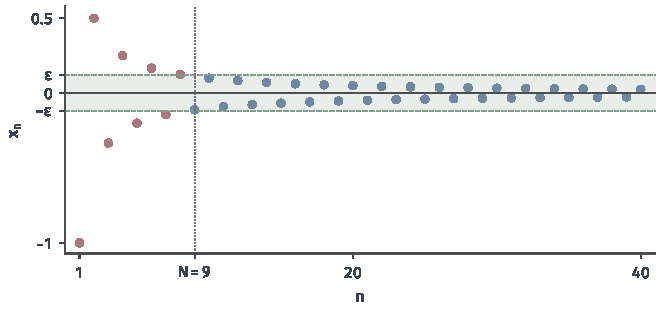
\includegraphics[width=112.0mm]{figures/01-mathematical-preliminaries-upper/01-mathematical-language-combinatorics-analysis-optimization/matplotlib/chapter3-concept-processes/sequence-tail.pdf}
 \caption{数列$x_n=(-1)^n/n$的前40项。绿色带为$|x_n|<0.12$，取$N=9$后，所有$n\geq9$都在带内；蓝点标记这个尾部，红点标记之前的项。尾部条件针对无限多个$n$，其成立依据是$1/n\leq1/9<0.12$，不是只检查图中有限个点。}
 \label{fig:analysis-process-sequence-tail}
\end{figure}

\subsection{数列的收敛判别}

定义收敛时需要指定一个候选极限，但很多数列的候选极限尚不明确。
下面依次利用变化方向、取值范围和尾部互近来判断极限是否存在，并说明各自需要的条件。

\subsubsection{单调数列的收敛}
若候选极限尚未确定，可以同时限制数列的变化方向和取值范围。
若对所有$n$都有$a_n\leq a_{n+1}$，称数列单调不减；
若总有$a_n\geq a_{n+1}$，称数列单调不增，两者统称为单调数列。

对于单调不减且有上界的数列，第~\ref{sec:prelim-optimal-values-errors}节的确界性质
为全部项提供一个最小上界；单调性将保证后面的项一直靠近它。
\begin{theorem}[单调有界收敛定理]
\label{thm:analysis-monotone-bounded-sequence}
设$(a_n)_{n\geq1}$为实数列。
若$a_n\leq a_{n+1}$对所有$n\geq1$成立，且存在$M\in\mathbb R$使$a_n\leq M$对所有$n\geq1$成立，则
\[
 \lim_{n\to\infty}a_n=\sup\{a_n:n\geq1\}\in\mathbb R.
\]
若$a_n\geq a_{n+1}$对所有$n\geq1$成立，且存在$m\in\mathbb R$使$a_n\geq m$对所有$n\geq1$成立，则
\[
 \lim_{n\to\infty}a_n=\inf\{a_n:n\geq1\}\in\mathbb R.
\]
\end{theorem}
\begin{proof}
设$a=\sup\{a_n:n\geq1\}$。给定$\varepsilon>0$，$a-\varepsilon$不是上界，
所以存在$N$使$a_N>a-\varepsilon$。单调性使$n\geq N$时都有
$a-\varepsilon<a_N\leq a_n\leq a$，这正是$a_n\to a$。
单调不增的情形对$-a_n$应用同一论证。
\end{proof}
这里使用实数\term{完备性}（completeness）的具体位置，是保证非空上有界实数集合的上确界仍为实数，
而不是另加一种数列变化条件。“有界”与“单调”也不能省去：$n$单调却无上界，
$(-1)^n$有界却不单调。

\subsubsection{有界数列的子序列收敛}
数列可能整体不收敛，但其中一些项仍有共同的趋向。保持原有次序选出一部分项，
得到子序列（subsequence），也称子列：若$n_1<n_2<\cdots$为严格递增的正整数列，
则$(a_{n_k})_{k\geq1}$为$(a_n)$的子序列。
收敛数列的每个子序列都收敛到同一极限，因为$n_k\to\infty$，原来的尾部误差界仍适用。
一个子序列收敛不能保证原数列收敛；$(-1)^n$的偶数项恒为$1$，奇数项恒为$-1$。

有界性不足以保证整列收敛，却能保证从中选出一个收敛子序列。
下面的结论称为Bolzano--Weierstrass定理，随后将用它证明柯西条件足以保证实数列收敛。
\begin{theorem}[Bolzano--Weierstrass定理]
\label{thm:analysis-bounded-subsequence}
设$(a_n)_{n\geq1}$为实数列。若存在$M\geq0$使$|a_n|\leq M$对所有$n\geq1$成立，
则存在严格递增的正整数列$n_1<n_2<\cdots$和$a\in\mathbb R$，使
\[
 \forall\varepsilon>0,\quad\exists K\in\{1,2,\ldots\},\quad
 k\geq K\Longrightarrow |a_{n_k}-a|<\varepsilon.
\]
即$a_{n_k}\to a$。
\end{theorem}
\begin{proof}
先取包含全部项的闭区间，将它平分，至少有一半仍包含无穷多项；
反复选择，得到嵌套闭区间$I_k=[l_k,r_k]$，每个区间都含无穷多项，长度为原长度的$2^{-k}$倍。
由$2^k\geq k+1$，这些长度至多为原长度的$1/(k+1)$，因而趋于零；这里不必先用后面的等比数列极限。
依次选取下标递增且$a_{n_k}\in I_k$的项。
由确界性质，$c=\sup_k l_k$满足$l_k\leq c\leq r_k$对每个$k$成立：
各$l_k$单调不减，而每个$r_k$都是所有左端点的上界。
给定$\varepsilon>0$，先选$K$使$r_K-l_K<\varepsilon$；
当$k\geq K$时，$a_{n_k}$与$c$同在$I_K$内，所以$|a_{n_k}-c|<\varepsilon$。
\end{proof}

\subsubsection{柯西数列的收敛}
单调条件并不适用于所有收敛数列。若还不知道候选极限，可以检查尾部各项是否彼此接近。
满足
\[
 \forall\varepsilon>0,\quad\exists N,\quad
 \forall m,n\geq N,\quad |a_m-a_n|<\varepsilon
\]
的数列称为\term{柯西数列}（Cauchy sequence）。
这个条件不指定候选极限，只比较尾部各项。对实数列，它与收敛等价。
\begin{theorem}[柯西收敛准则]
\label{thm:analysis-cauchy-convergence}
设$(a_n)_{n\geq1}$为实数列。存在$a\in\mathbb R$使$a_n\to a$，当且仅当
\[
 \forall\varepsilon>0,\quad\exists N\in\{1,2,\ldots\},\quad
 \forall m,n\geq N,\quad |a_m-a_n|<\varepsilon.
\]
\end{theorem}
\begin{proof}
每个收敛实数列都是柯西数列，因为
$|a_m-a_n|\leq|a_m-a|+|a_n-a|$，分别控制右侧两项即可。

反过来，柯西条件先保证数列有界：取误差$1$，尾部都在某一项两侧距离$1$以内，
有限个前项另取一个界即可。由上面的收敛子列结论，可取$a_{n_k}\to a$。
给定$\varepsilon>0$，先使任意$m,n\geq N$满足$|a_m-a_n|<\varepsilon/2$，
再选$n_k\geq N$使$|a_{n_k}-a|<\varepsilon/2$。
对每个$n\geq N$都有
$|a_n-a|\leq|a_n-a_{n_k}|+|a_{n_k}-a|<\varepsilon$。
\end{proof}
这一准则不必预先猜出极限；其充分性仍通过收敛子列依赖实数的确界性质。

验证柯西条件时，可把两个较晚的项之间的距离估计为逐步变化的总和。对$m>n$，
\begin{equation}
 |a_m-a_n|\leq\sum_{k=n}^{m-1}|a_{k+1}-a_k|.
\label{eq:analysis-cauchy-tail-bound}
\end{equation}
相邻差趋零还不够，因为中间的步数也在增加，必须控制整段和。
例如$a_1=0$、$a_{k+1}-a_k=1/k$时，每一步都趋零，但
$a_{2n}-a_n=\sum_{k=n}^{2n-1}1/k>1/2$，所以它不是柯西数列。
这一差别把极限问题引向下面的级数：单次贡献变小，并不等于全部贡献的累计稳定。

\subsection{极限的基本性质}

前面的判别给出了保证收敛的条件。现在假定实数列已经收敛，先检查极限的唯一性及数列的有界性，再分别计算和、差、数乘、积与商的极限，最后说明怎样用上下界夹逼求极限。
这些运算法则都以有限极限存在为前提，不能代替收敛性的判别。

\paragraph{极限的唯一性}
先假定极限存在，考察定义已经保证了什么。极限必唯一：若$a\neq b$都是极限，
取$\varepsilon=|a-b|/3$，充分靠后的项应同时满足
$|a_n-a|<\varepsilon$和$|a_n-b|<\varepsilon$；
三角不等式却给出$|a-b|\leq|a-a_n|+|a_n-b|<2|a-b|/3$，矛盾。

\paragraph{收敛数列的有界性}
收敛数列还必有界。取$\varepsilon=1$后，除有限个前项外都有$|a_n|\leq|a|+1$，
再把有限个前项的绝对值一并取最大值，即得到全列的界。
反向结论不成立，例如$(-1)^n$有界却不收敛；有界性只限制取值范围，没有控制尾部是否还在振荡。

\paragraph{和的极限}
实际计算时，一个数列常由几个已知数列相加得到。设$a_n\to a$、$b_n\to b$，其中$a,b\in\mathbb R$，则
\[
 \lim_{n\to\infty}(a_n+b_n)=a+b.
\]
因为$|(a_n+b_n)-(a+b)|\leq|a_n-a|+|b_n-b|$，
只需让两个误差分别小于$\varepsilon/2$，便能使和的误差小于$\varepsilon$。

\paragraph{差的极限}
相减时也可以分别控制两列数的误差。在同样的有限收敛条件下，
\[
 \lim_{n\to\infty}(a_n-b_n)=a-b.
\]
这来自$|(a_n-b_n)-(a-b)|\leq|a_n-a|+|b_n-b|$，取尾部起点使右侧两项各小于$\varepsilon/2$即可。

\paragraph{数乘的极限}
把每一项乘以固定的实数$c$，只会把误差乘以$|c|$，所以
\[
 \lim_{n\to\infty}ca_n=ca.
\]
$c=0$时结论直接成立；$c\neq0$时，把原数列误差控制在$\varepsilon/|c|$以内即可。

\paragraph{积的极限}
乘积的误差还包含一个变化的因子，因此先用收敛数列有界这一性质。若$a_n\to a$、$b_n\to b$，则
\[
 \lim_{n\to\infty}a_nb_n=ab.
\]
取$M\geq1$使所有$|a_n|\leq M$，分解误差得
\[
 |a_nb_n-ab|\leq M|b_n-b|+|b|\,|a_n-a|.
\]
让$|b_n-b|<\varepsilon/(2M)$、$|a_n-a|<\varepsilon/[2(|b|+1)]$同时成立，右侧便小于$\varepsilon$。

\paragraph{商的极限}
除法还须避免分母趋零。若$a_n\to a$、$b_n\to b$且$b\neq0$，则充分靠后的$b_n\neq0$，并且
\[
 \lim_{n\to\infty}\frac{a_n}{b_n}=\frac ab.
\]
事实上，充分靠后的$|b_n|\geq|b|/2$，于是
$|1/b_n-1/b|\leq2|b_n-b|/|b|^2\to0$，结合乘积规则即得结论。
例如将分子分母同除以$n$，可得$n/(n+1)\to1$。
这些运算法则针对已经存在的有限极限，不能把$0/0$或$\infty-\infty$直接当成数值计算。

\paragraph{夹逼定理}
有时中间数列不断振荡，直接控制它的误差并不方便，但可以分别找到上下界。
若上下两列最终都靠近同一有限值，中间数列便被限制在同一误差范围内。
\begin{theorem}[夹逼定理]
\label{thm:analysis-sequence-squeeze}
设$(a_n)$、$(b_n)$、$(c_n)$为实数列。若存在正整数$N_0$使
\[
 \forall n\geq N_0,\qquad a_n\leq c_n\leq b_n,
\]
并且存在$\ell\in\mathbb R$满足
$\lim_{n\to\infty}a_n=\lim_{n\to\infty}b_n=\ell$，则
$\lim_{n\to\infty}c_n=\ell$。
\end{theorem}
\begin{proof}
任给$\varepsilon>0$，由两端收敛可选正整数$N_1,N_2$，使
$n\geq N_1$时$|a_n-\ell|<\varepsilon$，$n\geq N_2$时$|b_n-\ell|<\varepsilon$。
取$N=\max\{N_0,N_1,N_2\}$，则每个$n\geq N$都有
\[
 \ell-\varepsilon<a_n\leq c_n\leq b_n<\ell+\varepsilon.
\]
所以$|c_n-\ell|<\varepsilon$，按定义即$c_n\to\ell$。
\end{proof}
例如$-1/n\leq(\sin n)/n\leq1/n$，所以$(\sin n)/n\to0$。

一个反复使用的例子是$|r|<1$时$r^n\to0$。$r=0$时直接成立；
若$0<|r|<1$，写$1/|r|=1+h$，其中$h>0$。
从$(1+h)^1=1+h$出发，每多乘一次$1+h$，都有
$(1+nh)(1+h)\geq1+(n+1)h$，所以$(1+h)^n\geq1+nh$。
因此$0<|r|^n\leq1/(1+nh)\to0$，再由夹逼定理得到结论。
这也给出式~\eqref{eq:prelim-geometric-recurrence}所定义等比递推的极限。

\subsection{数列的上极限与下极限}
有些数列既不收敛，也没有柯西性质；仍可考察它们尾部的上下边界。
为记录无界的趋向，约定$a_n\to+\infty$表示对每个实数$M$，充分大的$n$都满足$a_n>M$；
$a_n\to-\infty$则要求最终都有$a_n<M$。
这两个符号不是有限实数极限，$\overline{\mathbb R}=\mathbb R\cup\{-\infty,+\infty\}$称为扩展实数，
其中$\infty-\infty$没有定义。

逐渐舍去前项时，尾部下界只会上升，尾部上界只会下降，因此可以分别用单调极限记录它们。
\begin{definition}[数列的上极限与下极限]
\label{def:analysis-liminf-limsup}
对扩展实数列$(a_n)$，定义
\[
 \liminf_{n\to\infty}a_n
 =\lim_{n\to\infty}\inf_{k\geq n}a_k,
 \qquad
 \limsup_{n\to\infty}a_n
 =\lim_{n\to\infty}\sup_{k\geq n}a_k.
\]
右侧尾部下确界随$n$单调不减，尾部上确界随$n$单调不增，故两者的极限均在扩展实数中存在。
\end{definition}
例如$(-1)^n$的下极限为$-1$、上极限为$1$，通常极限不存在。
总有$\liminf a_n\leq\limsup a_n$；二者同为有限$a$当且仅当$a_n\to a$，
因为此时充分靠后的尾部上下边界可同时落在$a$附近，夹逼便控制了每个尾部项。
二者同为$+\infty$或$-\infty$时则对应上述无穷极限，仍应与有限实数收敛区别。
对有界实数列，上、下极限还是能够由子序列达到的极限：例如记$L=\limsup a_n$，
在足够晚的尾部内选一项大于$L-1/j$，并要求其下标超过前次所选的下标；
尾部上界又最终小于$L+1/j$，由此可构造趋于$L$的子列，下极限同理。

\subsection{级数的收敛}

\paragraph{级数与部分和}
把有限和的上限不断增大，就得到新的数列
\[
 s_N=\sum_{n=1}^{N}a_n=a_1+\cdots+a_N,
\]
$s_N$称为\term{部分和}（partial sum）。
符号\term{无穷级数}（infinite series）$\sum_{n=1}^{\infty}a_n$描述这一求和过程；
当$(s_N)$有有限极限$s$时，称级数收敛，并记$\sum_{n=1}^{\infty}a_n=s$。
例如$a_n=2^{-n}\to0$，但部分和$s_N=1-2^{-N}\to1$；
单项极限与级数的和是两个不同的对象。
由$a_N=s_N-s_{N-1}$可知，级数收敛必须有$a_N\to0$，反向则不成立，下面的$p=1$就是反例。

若所有$a_n\geq0$，部分和单调不减，因此有界时收敛，无界时趋于$+\infty$。
这种情形下统一记
\[
 \sum_{n=1}^{\infty}a_n:=\sup_N\sum_{n=1}^{N}a_n\in[0,+\infty].
\]
这是非负项级数的扩展总和；总和为$+\infty$时仍称级数发散，不把它混同于有限和。
非负项的累计没有正负抵消，因而可以直接比较不同部分和的大小。

\paragraph{几何级数}
第~\ref{chap:sets-functions-and-proofs}章的有限几何和公式~\eqref{eq:prelim-finite-geometric-sum}给出$r\neq1$时
\[
 \sum_{n=0}^{N}r^n=\frac{1-r^{N+1}}{1-r}.
\]
当$|r|<1$时，前面的等比数列极限使$r^{N+1}\to0$，因而
\begin{equation}
 \sum_{n=0}^{\infty}r^n=\frac{1}{1-r}.
\label{eq:analysis-geometric-series}
\end{equation}
同一计算给出截断后的误差
$|\sum_{n=N+1}^{\infty}r^n|=|r|^{N+1}/|1-r|$。
若$|r|\geq1$，单项$r^n$不趋零，故级数发散。
几何级数既是一个可直接计算的例子，也提供比较其他级数尾部的基准。

\paragraph{$p$级数}
对于$\sum_{n=1}^{\infty}n^{-p}$，相邻项的比值趋于$1$，仅看单步下降不易区分不同的$p$。
可以将有限和按$n=2^k,\ldots,2^{k+1}-1$分成区块。
若$p>0$，每块有$2^k$项，且
\[
 2^{-p}2^{k(1-p)}
 \leq\sum_{n=2^k}^{2^{k+1}-1}n^{-p}
 \leq2^{k(1-p)}.
\]
$p>1$时，右侧随$k$构成公比$2^{1-p}<1$的几何级数，故任意原部分和都有统一上界，
由非负部分和的单调性得到收敛。$0<p\leq1$时，每块至少为$2^{-p}$，累计任意多块便无界。
$p\leq0$时原级数的单项已不趋零。因此$p$级数恰在$p>1$时收敛；
特别地，调和级数$\sum_{n=1}^{\infty}1/n$发散。
区块上下界的来源是：块内每一项都介于$(2^{k+1})^{-p}$与$(2^k)^{-p}$之间，再乘以项数$2^k$。
任一部分和$s_N$都不超过包含它的前若干整块之和，所以对整块的估计控制了全部部分和。
这里只比较有限区块，尚未调用无穷级数的分组规则。

\subsubsection{级数的收敛判别}

判断级数收敛，就是判断部分和是否有有限极限。非负项的部分和单调，可以用上界控制；
出现正负项后，还须区分绝对值累计有限与依靠抵消才收敛的两种情形。

\paragraph{正项级数的收敛判别}
几何级数与$p$级数已提供两个基准。对一般正项级数，可以先比较单项，
再用非负部分和的单调性把大小关系传递到总和。
若充分大的$n$都有$0\leq a_n\leq b_n$，则
$\sum b_n$收敛蕴含$\sum a_n$收敛；$\sum a_n$发散蕴含$\sum b_n$发散。
这称为比较判别法，有限个前项不影响收敛。
例如$n\geq1$时$1/[n(n+1)]\leq1/n^2$，故其级数收敛。
若$a_n,b_n>0$且$a_n/b_n\to c\in(0,\infty)$，则最终
$(c/2)b_n\leq a_n\leq(3c/2)b_n$，两级数因而同收敛或同发散，称为极限比较判别法。

另一种比较从相邻项的比例入手。若$a_n>0$且$a_{n+1}/a_n\to r$，
当$r<1$时，可选$r<q<1$，使充分靠后都有$a_{n+1}\leq qa_n$，
逐次代入得到$a_{N+j}\leq a_Nq^j$，用几何级数比较便知收敛。
当$r>1$时，充分靠后的项递增而不趋零，级数发散；比值趋于$+\infty$亦同。
这称为比值判别法。$r=1$时无法据此判断：收敛的$\sum1/n^2$与发散的$\sum1/n$
都有相邻项比值趋于$1$，必须另用比较等方法。

\paragraph{变号级数的两种收敛}
项的正负交替或不规则变化时，部分和失去单调性，正负抵消也会影响累计。
若实数级数$\sum a_n$的绝对值级数$\sum|a_n|$收敛，称原级数
\term{绝对收敛}（absolute convergence）；若原级数收敛但$\sum|a_n|$发散，则称为条件收敛（conditional convergence）。
绝对收敛意味着即使不依赖抵消，累计的绝对贡献仍有限。
条件收敛则要求同时证明原级数收敛和绝对值级数发散；只知道后者，不能排除原级数也发散。

\paragraph{绝对收敛的判定}
先对非负项级数$\sum|a_n|$使用比较或比值判别，若其收敛，原级数便必收敛。
理由是对$m>n$有
\[
 |s_m-s_n|\leq\sum_{k=n+1}^{m}|a_k|,
\]
右侧作为收敛非负级数的一段尾和，能够对所有$m>n$同时趋于零，故$(s_n)$满足柯西准则。
因此实际判断时无需预先证明原级数收敛，再补查绝对值级数。
例如$\sum(-1)^{n+1}/n^2$由$p=2$的情形得到绝对收敛。
若级数和为$s$，相同估计给出
\[
 |s-s_N|\leq\sum_{n>N}|a_n|\longrightarrow0,
\]
将绝对尾和变为截断误差的上界。

\paragraph{条件收敛的判定}
绝对值级数发散后，还须判断原级数中的抵消是否足以使部分和稳定。
最基本的条件是：$b_n\geq0$单调不增且$b_n\to0$时，
交错级数$\sum_{n=1}^{\infty}(-1)^{n+1}b_n$收敛，这称为Leibniz判别法。
其偶数部分和单调不减，奇数部分和单调不增，且每个偶数部分和不超过任何其后的奇数部分和。
两列分别有界，故都有极限；两类相邻部分和之差为$b_{2n+1}\to0$，极限因而相同，
原部分和便收敛。级数和位于任意一对相邻的奇偶部分和之间，因此余项绝对值不超过$b_{N+1}$。
例如$\sum(-1)^{n+1}/n$收敛，绝对值级数却是调和级数，所以条件收敛。
若$\sum b_n$本来就收敛，Leibniz条件给出的交错级数则是绝对收敛，不能一概称为条件收敛。

更一般地，若$A_N=\sum_{n=1}^{N}a_n$一致有界，即存在$M$使$|A_N|\leq M$对所有$N$成立，
而$b_n\geq0$单调趋零，则$\sum a_nb_n$收敛，这称为Dirichlet判别法。
这里$a_n$提供有界振荡，$b_n$使振荡的权重趋零。
为说明二者如何配合，对$m\leq k$记$A_k^{(m)}=\sum_{n=m}^{k}a_n$，则$|A_k^{(m)}|\leq2M$。
把$a_k=A_k^{(m)}-A_{k-1}^{(m)}$代入有限和并整理，得到
\[
 \sum_{k=m}^{N}a_kb_k
 =A_N^{(m)}b_N+
   \sum_{k=m}^{N-1}A_k^{(m)}(b_k-b_{k+1}),
 \qquad A_{m-1}^{(m)}=0.
\]
因此尾部的绝对值不超过
$2M[b_N+\sum_{k=m}^{N-1}(b_k-b_{k+1})]=2Mb_m\to0$，由柯西准则得证。
取$a_n=(-1)^{n+1}$便回到交错情形。
该判别只保证原级数收敛；是否条件收敛，还须另外证明$\sum|a_nb_n|$发散。


图~\ref{fig:analysis-process-series-terms-sums}并排比较级数的项与部分和。两列项都趋零，累计后的行为仍然不同。
\begin{figure*}[!htbp]
 \centering
 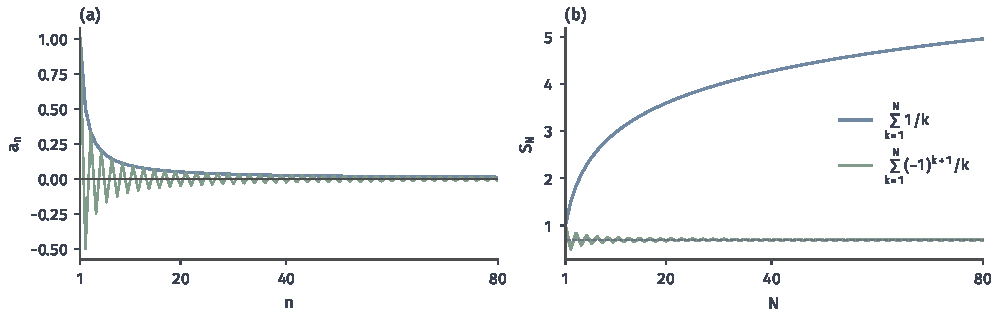
\includegraphics[width=169.0mm]{figures/01-mathematical-preliminaries-upper/01-mathematical-language-combinatorics-analysis-optimization/matplotlib/chapter3-concept-processes/series-terms-sums.pdf}
 \caption{(a) 蓝、绿折线分别连接$1/n$与$(-1)^{n+1}/n$的前80项。(b) 对应的部分和：调和部分和继续增长，交错调和部分和趋于虚线所示的$\log2$。项趋零只是级数收敛的必要条件；图展示有限段，收敛或发散由前面的判别证明。}
 \label{fig:analysis-process-series-terms-sums}
\end{figure*}

\subsubsection{级数的重排和分组对收敛的影响}

收敛判别确定了原次序下部分和的趋向。接下来改变求和的组织方式：重排改变各项的次序，
分组只把原次序中的有限个相邻项合并；两种操作对收敛性的影响不同，需要分别检验。

\paragraph{级数的重排}
有限和可以交换项的先后；无穷级数则要检查新的部分和如何覆盖旧项。
若$\pi:\{1,2,\ldots\}\to\{1,2,\ldots\}$为双射，$\sum_{n=1}^{\infty}a_{\pi(n)}$称为原级数的重排，
它每项恰好使用一次，改变的是各项进入累计的顺序。
对于非负项，任意有限选项的和都不超过原扩展总和；反过来，原来的任意前$N$项
也会全部进入重排的某个有限前段。对两个方向分别取上确界，便知重排保持总和，允许总和为$+\infty$。

绝对收敛也保证任意重排保持原和。
给定$\varepsilon>0$，先选$N$使$\sum_{n>N}|a_n|<\varepsilon$。
重排充分多项后已包含原来的前$N$项，而它选入或遗漏的其余贡献均来自这个绝对尾部。
将重排的有限和与原部分和比较，并让原部分和趋于$s$，误差至多为该绝对尾和，故重排仍趋于$s$。

条件收敛没有这一保证。设正项总和为$P$、负项绝对值总和为$Q$；
若其中一个有限，由$s_N=P_N-Q_N$收敛会推出另一个也有限，与绝对值和发散矛盾，
故二者都为$+\infty$。对任意实数目标$L$，可以依原先相对次序取正项直到部分和超过$L$，
再取负项直到低于$L$，反复进行；每次都至少取一项相应符号的项。
两类项最终都被用到，而$a_n\to0$使每次越过$L$的幅度趋零，因此可得到和为$L$的重排。
原级数若含零项，每轮再按原次序插入下一个尚未使用的零项（若有）；这不改变和，并保证每个零项也最终被用到。
也可交替超过$1$、低于$0$，构造不收敛的重排。
原来的和依赖抵消的顺序，不能只按有限和交换律任意调换。

\paragraph{级数的分组}
重排改变项的先后次序。若保留原次序，只将相邻的有限项合起来，则需要考察另一种改变求和方式的操作。
分组保持原项的顺序，只将有限个相邻项合为一项。
准确地说，取$0=n_0<n_1<n_2<\cdots$，令
$b_j=\sum_{k=n_{j-1}+1}^{n_j}a_k$，则分组后前$J$项的和恰为$s_{n_J}$。
所以原级数收敛到$s$时，分组后的部分和是原部分和的子序列，也必收敛到$s$；
这对绝对收敛和条件收敛都成立。

反向不成立。级数$1-1+1-1+\cdots$的部分和在$1$与$0$之间交替，原级数不收敛，
但按$(1-1)+(1-1)+\cdots$分组后各项为零。
分组只保留部分截断位置，可能掩盖块内的振荡。
非负项没有这种抵消：原部分和单调，分组截断又越过每一个原截断位置，
两者的上确界相同，故即使总和为$+\infty$也可保序分组。
结合非负重排规则，可先把非负项按任意编号排列，再分成有限相邻块，而不改变扩展总和；
后面的外测度构造将用这些求和性质累计覆盖区间的长度。

\FloatBarrier
\section{函数的极限}
\label{sec:analysis-function-limits}

数列的指标按自然数逐项增加，函数的输入却可以从许多实数位置靠近同一点。例如$(x^2-1)/(x-1)$在$x=1$没有定义，但在$x\neq1$时它等于$x+1$，所以邻近输入的输出仍趋于$2$。函数极限研究的正是这种去掉中心点后的共同趋近，不先要求函数在中心有取值。

\subsection{函数极限与单侧极限}
\paragraph{聚点}

讨论输入接近$a$之前，须保证定义域中确实有不同于$a$的输入能够任意靠近$a$。
设$X\subseteq\mathbb R$。若$a$的任意去心邻域都含有$X$中的点，
即每个$r>0$都能找到$x\in X$使$0<|x-a|<r$，就称$a$为$X$的聚点（cluster point）。
例如$0$是$(0,1)$的聚点，虽然$0$不属于这个集合；孤立点则不是聚点。
这个条件保证定义域中的点确实可以不断靠近$a$。

\paragraph{函数极限}
有了能够趋近的输入，还要用输入误差控制输出误差，这与数列极限比较尾部误差的思路相同。
设$f:X\to\mathbb R$，$a$为$X$的聚点。
若对每个$\varepsilon>0$，都存在$\delta>0$使
\[
 x\in X,\quad0<|x-a|<\delta\quad\Longrightarrow\quad|f(x)-b|<\varepsilon,
\]
就称$b$为$x\to a$时$f(x)$的极限，记作$\lim_{x\to a}f(x)=b$。
输入与$a$的距离足够小，便能保证输出与$b$的距离任意小。
定义中的$0<|x-a|$排除了中心点，所以既不要求$f(a)$有定义，也不要求它等于$b$。
例如$f(x)=(x^2-1)/(x-1)$在$x=1$没有定义，但对$x\neq1$有$f(x)=x+1$。
给定$\varepsilon>0$，取$\delta=\varepsilon$，则
$0<|x-1|<\delta$时$|f(x)-2|=|x-1|<\varepsilon$，所以其极限为$2$。


图~\ref{fig:analysis-process-epsilon-delta-band}将输入邻域与输出误差带对应起来，同时把基点取值与趋近时的极限分开。
\begin{figure}[!htbp]
 \centering
 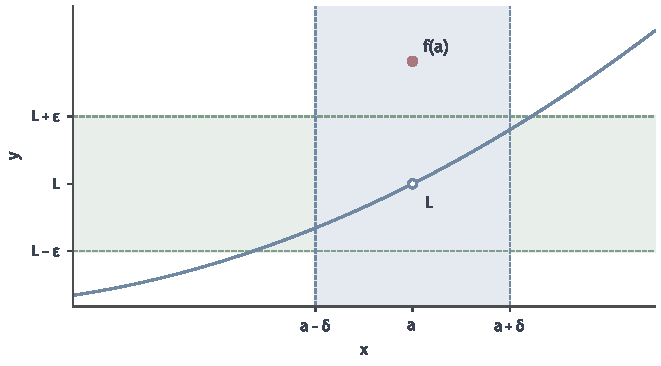
\includegraphics[width=112.0mm]{figures/01-mathematical-preliminaries-upper/01-mathematical-language-combinatorics-analysis-optimization/matplotlib/chapter3-concept-processes/epsilon-delta-band.pdf}
 \caption{取$a=L=1$，$x\neq1$时$f(x)=x^2$，另令$f(1)=2$。蓝带对应$\delta=0.2$的输入范围，绿带对应$\varepsilon=0.55$的输出范围；去掉$a$后，蓝带内曲线全部落在绿带内。空心点是极限位置，红实心点是$f(a)$，不参加去心邻域条件。}
 \label{fig:analysis-process-epsilon-delta-band}
\end{figure}

\paragraph{左极限与右极限}
实轴上的输入可以从一个点的两侧接近，而两侧的输出未必有相同趋向，因此先分别考察每一侧的极限。
只让$x<a$的点趋近$a$，得到左极限$\lim_{x\uparrow a}f(x)$；
只让$x>a$的点趋近$a$，得到右极限$\lim_{x\downarrow a}f(x)$。
两种定义分别在上述误差条件中增加$x<a$或$x>a$，
并要求相应一侧存在定义域中的点任意靠近$a$。
若两侧都能趋近$a$，双侧极限存在当且仅当左右极限都存在且相等。
例如$f(x)=\mathbb I\{x\geq0\}$在$0$处的左右极限分别为$0$和$1$，所以双侧极限不存在。
这里$\mathbb I$为指示函数：括号内条件成立时取$1$，否则取$0$。
在定义域$[a,b]$内，只能从右侧趋近左端点$a$，从左侧趋近右端点$b$。
这种左右判据依赖实轴上的顺序，多元函数还须控制其他趋近方式。

\paragraph{无穷远处的极限}
输入也可以趋于无穷。设定义域向右无界，条件
\[
 \lim_{x\to+\infty}f(x)=b
\]
表示：对每个$\varepsilon>0$，存在$M$，使定义域中所有$x>M$都满足$|f(x)-b|<\varepsilon$。
定义域向左无界时，$x\to-\infty$的定义相应要求所有$x<M$的允许输入满足同一误差界。
例如$1/x$在$x\to+\infty$和$x\to-\infty$时都趋于$0$。

\paragraph{值为无穷的极限}
前一段改变的是输入的趋向；即使输入趋近有限点，输出也可能越过任何有限界，因此还需要描述输出本身的无界趋向。
对有限聚点$a$，$f(x)\to+\infty$（$x\to a$）是指：对每个实数$M$，都存在$\delta>0$，使定义域中满足$0<|x-a|<\delta$的每个$x$都有$f(x)>M$。
趋于$-\infty$则把最后的不等式改为$f(x)<M$。单侧无穷极限再限制输入所在的一侧。因此$1/x$在$x\downarrow0$时趋于$+\infty$，在$x\uparrow0$时趋于$-\infty$，并没有共同的双侧无穷极限。

\subsection{常用极限}

\paragraph{三角函数的基本极限}
三角函数的自变量采用弧度制：单位圆上弧长为$h$的圆心角记为$h$。
比较内接三角形、扇形和外切三角形的面积，可得$0<h<\pi/2$时
$\sin h\leq h\leq\tan h$，从而$\cos h\leq\sin h/h\leq1$。
又由$1-\cos h=2\sin^2(h/2)\leq h^2/2$得到误差界
\[
 0\leq1-\frac{\sin h}{h}\leq1-\cos h\leq\frac{h^2}{2}.
\]
任给$\varepsilon>0$，只要$0<h<\min\{\pi/2,\sqrt{2\varepsilon}\}$，第一个比值与$1$的误差就小于$\varepsilon$。
同样由$|1-\cos h|/|h|\leq|h|/2$可控制第二个比值。因此
\[
 \lim_{h\to0}\frac{\sin h}{h}=1,
 \qquad
 \lim_{h\to0}\frac{\cos h-1}{h}=0.
\]
第一个比值是偶函数，所以右侧的论证也控制$h<0$；第二个误差界对正负两侧都适用。
弧度制使第一个极限恰为$1$，用角度制时会多出比例系数。

\paragraph{自然指数函数}
后面求指数函数的导数需要一个原点处的基本极限，因此先用级数构造自然指数函数，验证其收敛，再建立乘法性质和局部变化关系。
自然指数函数可由绝对收敛的级数构造：
\[
 \exp x=\sum_{k=0}^{\infty}\frac{x^k}{k!}.
\]
对固定$x$，充分靠后的相邻项绝对值之比不超过$1/2$，尾部被几何级数控制，所以级数收敛。
设两个级数的项分别为$a_k$与$b_j$。有限矩形和满足
$\sum_{k=0}^N\sum_{j=0}^Ma_kb_j=(\sum_{k=0}^Na_k)(\sum_{j=0}^Mb_j)$，
所以它们趋于两级数和的乘积。若两个级数都绝对收敛，双重和中各项的绝对值总和
由$(\sum_k|a_k|)(\sum_j|b_j|)$控制；舍去足够大的有限矩形后，剩余绝对尾和可任意小。
因此按总次数$k+j$合并，也得到同一极限。把这个结论用于指数级数，记
$C_n=\sum_{k=0}^n x^ky^{n-k}/[k!(n-k)!]$。将系数$n$拆为$k+(n-k)$，并分别换一次有限求和的索引，得到
\[
 nC_n=(x+y)C_{n-1},\qquad n\geq1.
\]
由$C_0=1$逐步得到$C_n=(x+y)^n/n!$，因而
\[
 \exp x\,\exp y
 =\sum_{n=0}^{\infty}\sum_{k=0}^n\frac{x^ky^{n-k}}{k!(n-k)!}
 =\sum_{n=0}^{\infty}\frac{(x+y)^n}{n!}
 =\exp(x+y).
\]
记$e=\exp1$，则$\exp x$就是以$e$为底的指数函数，通常写作$e^x$；$e$约为$2.71828$。
当$0<|h|<1/2$时，直接估计级数的二阶以后各项：
\[
 |e^h-1-h|
 \leq\sum_{k=2}^{\infty}|h|^k
 =\frac{h^2}{1-|h|}\leq2h^2.
\]
除以$|h|$并取极限，就有
\[
 \lim_{h\to0}\frac{e^h-1}{h}=1.
\]
这一推导先用级数构造指数函数，未使用求导或积分。
加法公式给出$e^xe^{-x}=1$以及$e^x=(e^{x/2})^2$，因此$e^x>0$。
对$u\geq0$，级数各项非负，只保留前两项便得
\[
 e^u\geq1+u\qquad(u\geq0),
\]
这正是第~\ref{chap:combinatorics}章简化Sauer--Shelah界时所用的不等式。
对$h>0$，由此$e^h\geq1+h>1$，于是$e^{x+h}=e^xe^h>e^x$，指数函数严格递增。
同一估计说明$x\to+\infty$时$e^x\to+\infty$；取倒数又得$x\to-\infty$时$e^x\to0$。
对固定$x$，上述余项界还给出$|e^{x+h}-e^x|\leq e^x(|h|+2h^2)\to0$。
这些性质将在连续函数的介值定理建立后，用于构造自然对数这一反函数
\scite{math-lebl-analysis1}。

\subsection{极限的性质与运算}
\paragraph{序列判据}

函数极限要求控制$a$附近所有允许的输入。这个条件等价于：每列满足$x_n\in X\setminus\{a\}$且$x_n\to a$的输入，都有$f(x_n)\to b$。正向把函数极限的同一个$\delta$用于序列尾部即可。反向若误差条件不成立，就存在$\varepsilon_0>0$，使每个$1/n$邻域内都能选到$x_n\neq a$，满足$|f(x_n)-b|\geq\varepsilon_0$；这列输入趋于$a$，输出却不趋于$b$，与序列条件矛盾。

\paragraph{和的极限}
序列判据把函数极限转化为数列极限，从而可以逐项建立函数极限的运算法则。
以下各段统一设$f,g:D\to\mathbb R$，$a$为$D$的聚点，且在$x\in D$、$x\to a$时
$f(x)\to b$、$g(x)\to c$，其中$b,c\in\mathbb R$。和的极限为
\[
 \lim_{x\to a}(f(x)+g(x))=b+c.
\]
任取$x_n\in D\setminus\{a\}$且$x_n\to a$，序列判据给出$f(x_n)\to b$、$g(x_n)\to c$；
数列和的法则给出$f(x_n)+g(x_n)\to b+c$。由于对任意这样的输入列都成立，再用序列判据即得结论。

\paragraph{差的极限}
相减也保留有限极限关系：
\[
 \lim_{x\to a}(f(x)-g(x))=b-c.
\]
对每列趋于$a$的允许输入，数列差的法则都给出相应输出差趋于$b-c$，再由序列判据返回函数极限。

\paragraph{数乘的极限}
固定倍数只按比例改变输出误差。对任意固定$\lambda\in\mathbb R$，
\[
 \lim_{x\to a}\lambda f(x)=\lambda b.
\]
沿任意允许输入列使用数列常数倍的极限，再用序列判据即可；$\lambda=0$时输出恒为零。

\paragraph{积的极限}
两个有限极限也可以分别相乘：
\[
 \lim_{x\to a}f(x)g(x)=bc.
\]
沿任意允许输入列应用数列乘积的法则，得到输出积趋于$bc$；序列判据保证这控制了$a$附近的全部允许输入。

\paragraph{商的极限}
商需要额外要求分母极限$c\neq0$，此时
\[
 \lim_{x\to a}\frac{f(x)}{g(x)}=\frac bc.
\]
先取输出误差$|c|/2$，便知$a$的某个去心邻域内有$|g(x)|>|c|/2>0$，商在那里有定义。
在这一邻域内，任意输入列都可使用数列的商法则，再由序列判据得到结论。
若分子分母都趋于零，就不能套用此式。例如$(x^2-1)/(x-1)$在$x\to1$时须先约去公因子$x-1$，才能求出极限$2$。
同样，$\infty-\infty$等形式也须先变形或另外估计。

\paragraph{夹逼定理}
不易直接分解的函数，可以用同趋向的两侧函数控制。设在$a$的某个去心邻域内，所有允许输入满足
$u(x)\leq h(x)\leq v(x)$，且$u(x)\to L$、$v(x)\to L$，其中$L\in\mathbb R$，则
\[
 \lim_{x\to a}h(x)=L.
\]
任给$\varepsilon>0$，取一个共同的输入邻域，使$u(x)$和$v(x)$都落在$(L-\varepsilon,L+\varepsilon)$内，
中间的$h(x)$也在其中。例如$-|x|\leq x\sin(1/x)\leq|x|$在$x\neq0$时成立，因此$x\to0$时$x\sin(1/x)\to0$。

\subsection{无穷小与无穷大}

\paragraph{无穷小}
趋向零的量可以出现在数列、函数或后面的微分余项中，先给这类趋向一个统一名称。
在指定的趋向下，极限为$0$的函数称为无穷小（infinitesimal）。
例如$x\to0$时，$x$和$x^2$都是无穷小；$n\to\infty$时，$1/n$也是无穷小。
“无穷小”描述变化过程中的极限性质，不是某个固定的很小的非零数。

\paragraph{无穷大}
函数值的绝对值也可能最终超过任意固定门槛，这种趋向与趋零可以通过倒数联系起来。
在指定的趋向下，若$|f(x)|\to+\infty$，则称$f$为无穷大。
例如$x\to0$时，$1/x$为无穷大，但它没有共同的正或负无穷极限。
若$f$在所考察范围内非零，则$|f|\to\infty$等价于$1/f\to0$。

\paragraph{渐近记号}
\label{sec:comb-growth-scales}
两个函数即使同为无穷小，趋零的相对速度也可以不同。
设在所讨论的趋向附近$g\neq0$，定义
\[
 f=o(g)\quad\text{表示}\quad \frac{f}{g}\longrightarrow0.
\]
这个小$o$记号表示$f$相对于$g$可以忽略。
若$|f/g|$在趋向附近有界，则记$f=O(g)$，称为大$O$记号。
大$O$只要求有常数$C$使$|f|\leq C|g|$最终成立，小$o$则要求这个相对比例趋于零。
例如$x\to0$时$x^2=o(x)$，而$3x=O(x)$但不是$o(x)$。
若$f/g\to1$，还记$f\sim g$，称为等价无穷小（当两者都趋零时）。
例如$x+x^2\sim x$，因为$(x+x^2)/x=1+x\to1$。

同样的记号可用于$n\to\infty$的数列：
$3n+7=O(n)$、$n/10=O(n)$，但这两个比值分别趋于$3$和$0.1$，所以都不是$o(n)$；
$10\sqrt n=o(n)$，因为$10\sqrt n/n=10/\sqrt n\to0$。
图~\ref{fig:vol1-add-asymptotic-ratios}画出这三个比值。

\begin{figure}[!htb]
  \centering
  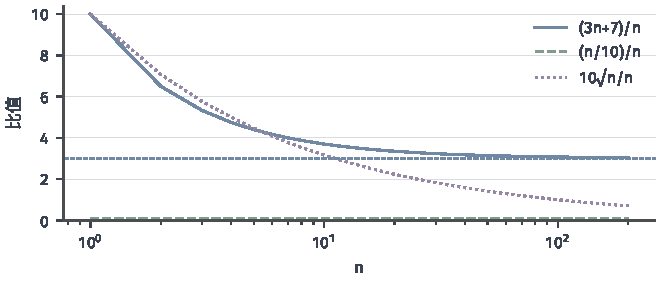
\includegraphics[width=112mm]{figures/01-mathematical-preliminaries-upper/01-mathematical-language-combinatorics-analysis-optimization/matplotlib/comprehension-additions/asymptotic-ratios.pdf}
  \caption{三个解析数列除以$n$后的比值，展示整数$n=1,\ldots,200$，横轴为对数刻度。蓝、绿、紫线的极限分别为$3,0.1,0$。前两者对应$O(n)$而非$o(n)$，第三者对应$o(n)$；极限由正文中的表达式判断，有限范围曲线只帮助观察。}
  \label{fig:vol1-add-asymptotic-ratios}
\end{figure}

对最终为正的数列，若存在$c>0$使$a_n\geq cb_n$最终成立，记$a_n=\Omega(b_n)$；
同时满足$a_n=O(b_n)$与$a_n=\Omega(b_n)$，记$a_n=\Theta(b_n)$，表示同一数量级。
例如$3n+7=\Theta(n)$。这里的常数不随趋于无穷的$n$改变。
$n=O(n^2)$也成立，因此大$O$给出上界，不一定给出精确的增长阶。
这些记号在求导和局部近似中用来表达余项的大小。

\FloatBarrier

\section{实数集与欧氏空间中的邻域和闭区间}
\label{sec:analysis-metric-measurement}
\label{sec:analysis-set-metric}

前两节的数列极限与函数极限都在控制距离：$|a_n-a|<\varepsilon$说明第$n$项离极限不远，
$0<|x-a|<\delta$说明输入离中心不远。本节先在实轴和有限维欧氏空间中把“一个点附近”写成开球与邻域，
再用邻域定义开集、闭集，并用点列刻画闭性；最后建立闭区间的有限子覆盖性质。
这些结论直接服务于下一章一元函数的连续性和极值，也服务于多元微积分中的欧氏集合。
把绝对值和欧氏范数抽象成任意集合上的度量，再讨论一般空间的完备性、可分性、全有界和紧致序列刻画，
是第~\ref{chap:metric-spaces}章“度量空间”的任务；本节不预设一般度量空间的结论。

\subsection{开球、邻域与开闭集}

\paragraph{开球与邻域}
讨论一个点附近的变化，需要先指定哪些对象算作离它足够近。给定中心和距离阈值后，可以把这些对象收集成一个集合。

\begin{definition}[欧氏开球]
\label{def:analysis-open-ball}
在$\mathbb R^d$中，以$\bm{x}$为中心、半径$r>0$的\term{开球}（open ball）记为
$B(\bm{x},r)=\{\bm{y}\in\mathbb R^d:\lVert\bm{y}-\bm{x}\rVert_2<r\}$。
当$d=1$时，$B(x,r)=(x-r,x+r)$就是开区间。
\end{definition}

开球把“离一个点足够近”写成集合。若集合$V$包含某个$B(\bm{x},r)$，就称$V$是$\bm{x}$的邻域；
邻域本身不必是开集。由这些邻域可以判断一个范围是否包含其中每个点附近的点。

图~\ref{fig:analysis-ball-neighborhood}将这两个对象分开：开球由距离直接确定，邻域则只需包含一个这样的开球。
\begin{figure}[htbp]
 \centering
 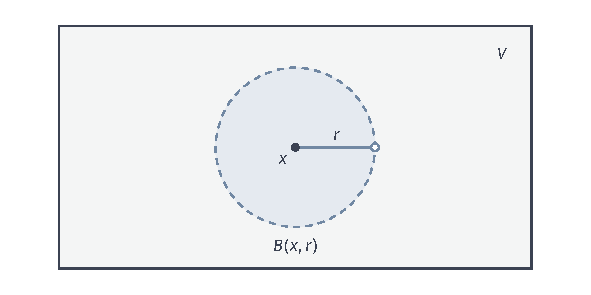
\includegraphics[width=\linewidth]{figures/01-mathematical-preliminaries-upper/01-mathematical-language-combinatorics-analysis-optimization/tikz/metric-ball-neighborhood/figure.pdf}
 \caption{平面欧氏距离下的开球与邻域。浅蓝圆盘为$B(\bm{x},r)$，虚线圆周不属于开球；灰色矩形$V$连同实线边界包含这个圆盘，因此是$\bm{x}$的邻域。$V$本身不是开集，说明“是某点的邻域”只要求在该点周围留有余量。}
 \label{fig:analysis-ball-neighborhood}
\end{figure}

\paragraph{开集与闭集}
有了开球，就能检验一个集合是否容纳其中每个点附近的一小片范围。对集合的补集作同样检验，又得到另一类常用的范围条件。

\begin{definition}[开集与闭集]
\label{def:analysis-open-closed-sets}
在$\mathbb R^d$中，集合$U$若对每个$\bm{x}\in U$都存在$r>0$使$B(\bm{x},r)\subseteq U$，就称为\term{开集}（open set）；
集合$F$若其补集$\mathbb R^d\setminus F$为开集，就称为\term{闭集}（closed set）。
\end{definition}

开闭性总是相对于当前空间而言。例如$[0,1/2)$在$\mathbb R$中不是开集，
但在子空间$X=[0,1]$中是开集：此时开球是实轴开区间与$X$的交，
$0$的一个小球不必包含负数。全集和空集既开又闭；“不是开集”也不等于“就是闭集”，实轴上的$[0,1)$便两者都不是。

图~\ref{fig:analysis-open-closed-relative}用端点附近的小球检验上述区别：实轴上包含端点的区间可能无法容纳小球，而在子空间中，小球本身也会随空间改变。
\begin{figure*}[htbp]
 \centering
 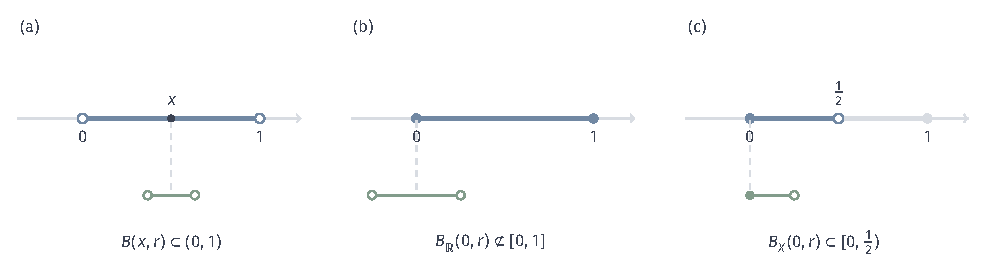
\includegraphics[width=169mm]{figures/01-mathematical-preliminaries-upper/01-mathematical-language-combinatorics-analysis-optimization/tikz/metric-open-closed-relative/figure.pdf}
 \caption{开集、闭集与所在空间。蓝色线段为待检验集合，绿色线段示意小球，空心端点排除、实心端点包含。(a) 在$\mathbb R$中，$(0,1)$的每个点都能选取一个包含于集合的小球，故为开集。(b) $[0,1]$在端点$0$处不能容纳任何实轴小球，因而不是开集；其补集$(-\infty,0)\cup(1,\infty)$为开集，故它是闭集。(c) 改在$X=[0,1]$中取球时，$B_X(0,r)=[0,r)$（$0<r<1/2$），因此$[0,1/2)$是$X$中的开集。图中只画出(c)的端点检验，其余点可直接沿用区间内部的小球。}
 \label{fig:analysis-open-closed-relative}
\end{figure*}

开球本身确实是开集：若$\bm{y}\in B(\bm{x},r)$，取$\rho=r-\lVert\bm{y}-\bm{x}\rVert_2>0$，
则三角不等式保证$B(\bm{y},\rho)\subseteq B(\bm{x},r)$。
任意多个开集的并仍开，因为并集中每个点都已属于某一个开集，可以沿用它的小球；
有限个开集的交仍开，因为可取各个允许半径的最小值。
无限多个开集的交则未必开，例如$\bigcap_{n\geq1}(-1/n,1/n)=\{0\}$。

\subsection{闭集的序列判据}

在欧氏空间中，闭集也可以用点列极限是否留在集合内来刻画。
$\mathbb R^d$中的点列$(\bm{x}_n)$收敛到$\bm{x}$，是指$\lVert\bm{x}_n-\bm{x}\rVert_2\to0$；
由于
\[
  |x_{n,j}-x_j|\leq\lVert\bm{x}_n-\bm{x}\rVert_2
  \leq\sqrt d\max_{1\leq j\leq d}|x_{n,j}-x_j|,
\]
欧氏距离收敛与有限个坐标同时收敛等价。

\begin{lemma}[闭集的序列判据]
\label{lem:analysis-closed-sequence-criterion}
设$F$为$\mathbb R^d$中的集合。$F$是闭集，当且仅当：对每个取值于$F$的点列$(\bm{x}_n)$，
若$\bm{x}_n\to\bm{x}$在$\mathbb R^d$中成立，则$\bm{x}\in F$。
\end{lemma}
\begin{proof}
若$F$闭而$\bm{x}\notin F$，开集$\mathbb R^d\setminus F$包含某个$B(\bm{x},r)$。
收敛要求充分靠后的$\bm{x}_n$落入这个球，与$\bm{x}_n\in F$矛盾。
反之，若$F$不闭，则存在$\bm{x}\in\mathbb R^d\setminus F$，使每个$B(\bm{x},r)$都与$F$相交。
为每个$n$选$\bm{x}_n\in F\cap B(\bm{x},1/n)$，便有$\bm{x}_n\to\bm{x}\notin F$，违反序列条件。
\end{proof}

例如$(0,1)$中的$1/n$在$\mathbb R$中趋于$0$，而$0\notin(0,1)$，所以$(0,1)$不是实轴中的闭集；
改在子空间$(0,1)$中判断时，$0$已不是环境中的候选极限。闭与有界描述的也是不同性质：
$(0,1)$有界但不闭，$\mathbb R$闭但不有界。

\subsection{闭区间的有限子覆盖性质}

\paragraph{开覆盖与有限子覆盖}

连续性在每一点给出一个邻域内的控制，但不同点的邻域大小可能不同。
要得到对整个闭区间同时有效的结论，需要从无限多个邻域中选出有限个，仍覆盖整个区间；
测量区间长度时也会遇到同样的问题：用可数多个开区间覆盖闭区间后，希望只保留其中有限个。
下面先规定“从一族开集中选出有限部分仍不遗漏”的含义。
\begin{definition}[开覆盖与紧致性]
\label{def:analysis-compactness}
设$K\subseteq\mathbb R^d$。一族开集的并包含$K$时，称它们为$K$的\term{开覆盖}（open cover）；
从中选出的有限个开集仍覆盖$K$时，称它们构成\term{有限子覆盖}（finite subcover）。
若$K$的每个开覆盖都存在有限子覆盖，则称$K$\term{紧致}（compact）。
\end{definition}
开覆盖本身可以有无限多个成员；有限子覆盖要求从原来的成员中挑选，而不是另换一组集合。

\paragraph{闭区间的紧致性}

闭区间里的点不会逃向无穷，收敛子列的极限也不会离开区间。
这两个条件使局部邻域覆盖不能一直要求加入新的成员。
\begin{theorem}[闭区间的有限子覆盖性质]
\label{thm:analysis-interval-finite-subcover}
实轴上的每个闭区间$[a,b]$都是紧致集。
\end{theorem}
\begin{proof}
$a=b$时选择一个包含该点的覆盖成员即可。设$a<b$，并给定$[a,b]$的开覆盖$\mathcal U$。
先证明这组覆盖有一个共同尺度：
\begin{equation}
 \exists r>0,\quad\forall x\in[a,b],\quad\exists U\in\mathcal U,
 \qquad B(x,r)\cap[a,b]\subseteq U.
\label{eq:analysis-cover-uniform-radius}
\end{equation}
若不存在这样的$r$，对每个$n$可选$x_n\in[a,b]$，使
$B(x_n,1/n)\cap[a,b]$不包含于任何一个覆盖成员。
有界数列$(x_n)$有子列$x_{n_k}\to x\in[a,b]$。
选$U\in\mathcal U$包含$x$，由开性取$\rho>0$使$B(x,\rho)\subseteq U$。
当$k$足够大时，$|x_{n_k}-x|<\rho/2$且$1/n_k<\rho/2$，
于是$B(x_{n_k},1/n_k)\subseteq B(x,\rho)\subseteq U$，产生矛盾。

有了共同半径$r$，把$[a,b]$分成有限个长度小于$r$的小区间。
每段任选一个点$x$，整段都落在$B(x,r)\cap[a,b]$内，故可由一个覆盖成员包含。
每段选择一个这样的成员，得到有限子覆盖。
\end{proof}

每个有界闭集$K\subseteq\mathbb R$也有此性质：先把它放入某个$[a,b]$，
再把$\mathbb R\setminus K$加入它的任意开覆盖，应用闭区间结论后删去这一补集。
在有限维欧氏空间$\mathbb R^d$中，闭且有界的集合同样紧致：逐次对各坐标使用Bolzano--Weierstrass定理，
可以从任意有界点列中选出在$\mathbb R^d$内收敛的子列，闭集的序列判据再把极限留在集合内；
这一序列刻画与开覆盖紧致性在一般度量空间中的等价证明，留到第~\ref{chap:metric-spaces}章。
有限子覆盖控制的是整个集合，而非只在几个已选点附近留出余量。图~\ref{fig:analysis-process-finite-open-cover}对照一个闭区间的有限覆盖与一个开区间上无法有限选取的覆盖族。
\begin{figure}[!htbp]
 \centering
 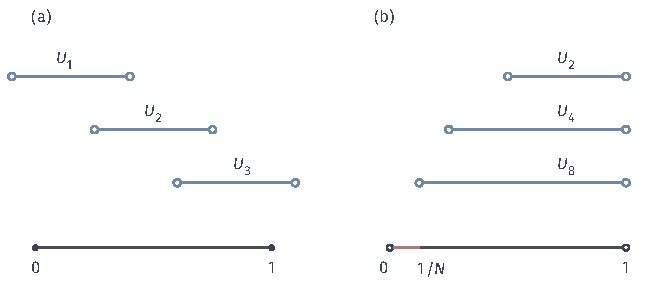
\includegraphics[width=112mm]{figures/01-mathematical-preliminaries-upper/01-mathematical-language-combinatorics-analysis-optimization/tikz/chapter3-concept-processes/finite-open-cover.pdf}
 \caption{(a) 三个开区间$(-0.1,0.4)$、$(0.25,0.75)$、$(0.6,1.1)$覆盖$[0,1]$。(b) $U_n=(1/n,1)$（$n\geq2$）覆盖$(0,1)$；只选有限多个时，设最大下标为$N$，红段$(0,1/N]$仍未覆盖。图只画$U_2,U_4,U_8$；右侧的失败由最大下标论证，不是有限图像的猜测。}
 \label{fig:analysis-process-finite-open-cover}
\end{figure}

\FloatBarrier


\FloatBarrier
\section{本章小结}
\label{sec:function-limits-summary}

$|\rho|<1$时等比序列趋于零，有限几何和趋于$1/(1-\rho)$。
极限先规定趋近的含义，再分别研究怎样计算极限、怎样保证极限存在；后者依赖实数的确界原理。
级数把累计过程写成部分和的极限；重排改变项的顺序，分组保留次序而合并相邻项，二者的结论不能混用。
度量规定点之间的距离，开集、闭集、完备性与紧致性由距离描述。
闭区间的紧致性使局部控制能够合成整体控制，后续微积分将据此研究连续性、变化与累计。
